\chapter{RESULTADOS PRELIMINARES DEL ENTRENAMIENTO}

\section{Arquitectura multimodelo evaluada}

La solución no depende de un único algoritmo. Se entrenaron trece configuraciones: cuatro para precio FOB, cuatro para margen, cuatro para riesgo y un ensamble FOB. El ensamble promedia Random Forest, HistGradientBoosting, ElasticNet y Prophet sin ajustar sus pesos sobre el conjunto de prueba.

\begin{table}[H]
\centering
\caption{Uso de los modelos en las cinco soluciones propuestas}
\label{tab:arquitectura_multimodelo}
\begin{singlespace}
\scriptsize
\renewcommand{\arraystretch}{1.05}
\begin{tabular}{p{2.7cm}p{4.1cm}p{5.6cm}}
\toprule
\textbf{Solución} & \textbf{Modelos utilizados} & \textbf{Resultado consumido por el módulo} \\
\midrule
S-1 Rentabilidad & Random Forest, HistGradientBoosting, ElasticNet y Prophet. & Margen estimado en S/kg a partir del precio, rendimiento, porcentaje vendido y ubicación. \\
S-2 Escenarios & Random Forest, HistGradientBoosting, regresión logística y Prophet. & Probabilidad de margen bajo y clasificación de escenarios optimista, esperado y pesimista. \\
S-3 Predicción FOB & Random Forest, HistGradientBoosting, ElasticNet, Prophet y ensamble. & Precio FOB esperado a seis semanas y dispersión entre modelos. \\
S-4 Histórico interactivo & Los cuatro modelos FOB y los datos observados. & Comparación temporal entre precio real, pronósticos y errores por periodo. \\
S-5 Reportes de ciclos & Ensamble FOB, modelos de margen y modelos de riesgo. & Síntesis de tendencias, periodos favorables, alertas y diferencias entre algoritmos. \\
\bottomrule
\end{tabular}
\end{singlespace}
\end{table}

Las soluciones S-4 y S-5 no requieren entrenar un algoritmo adicional. Son capas descriptivas y de comunicación que reutilizan los datos históricos y las salidas de todos los modelos. Esta separación evita confundir una función de visualización o reporte con un nuevo modelo predictivo.

\section{Conjuntos de datos obtenidos}

La ejecución reproducible de los scripts generó tres conjuntos analíticos. El conjunto de predicción FOB contiene 2\,312 observaciones válidas con precio objetivo localizado aproximadamente seis semanas después de cada observación inicial. Se reservaron cronológicamente 1\,849 registros para entrenamiento y 463 para prueba. El conjunto de margen contiene 585 registros relacionados con mercado exterior; 438 se utilizaron para entrenamiento y 147 para prueba. El conjunto de escenarios contiene las mismas 585 observaciones, de las cuales 147 pertenecen al cuartil inferior del margen y fueron etiquetadas como riesgo de margen bajo.

La reducción del conjunto FOB respecto del archivo original se debe a que se eliminaron filas sin una observación futura dentro de una tolerancia de dos semanas alrededor del horizonte solicitado. Así se evita interpretar seis registros posteriores como si fueran necesariamente seis semanas.

\section{Predicción del precio FOB a seis semanas}

\begin{table}[H]
\centering
\caption{Métricas de los modelos de precio FOB}
\label{tab:resultados_fob}
\small
\begin{tabular}{lrrrr}
\toprule
\textbf{Modelo} & \textbf{MAE} & \textbf{RMSE} & \textbf{MAPE (\%)} & \textbf{$R^2$} \\
\midrule
Random Forest & 0,321 & 0,425 & 19,482 & 0,247 \\
HistGradientBoosting & \textbf{0,319} & 0,426 & \textbf{19,001} & 0,245 \\
ElasticNet & 0,331 & \textbf{0,421} & 20,854 & \textbf{0,264} \\
Prophet & 0,410 & 0,503 & 22,009 & -0,055 \\
\textbf{Ensamble de cuatro modelos} & \textbf{0,314} & \textbf{0,400} & \textbf{18,339} & \textbf{0,333} \\
\bottomrule
\end{tabular}
\end{table}

Entre los modelos individuales, HistGradientBoosting obtuvo el menor MAE y MAPE, mientras que ElasticNet alcanzó el menor RMSE y el mayor $R^2$. Prophet, después de incorporar el precio FOB actual, la semana, el volumen, los rezagos, el promedio móvil, el destino y la temporada, redujo su error respecto de la configuración inicial, aunque todavía presentó menor capacidad explicativa que los otros modelos individuales.

El mejor resultado global corresponde al ensamble de los cuatro modelos. Frente al mejor modelo individual, redujo el MAE de 0,319 a 0,314 USD/kg y el MAPE de 19,001\,\% a 18,339\,\%. Asimismo, disminuyó el RMSE de 0,421 a 0,400 USD/kg y elevó el $R^2$ de 0,264 a 0,333. La mejora indica que los errores de Prophet y de los modelos de aprendizaje automático no coinciden completamente; al promediarlos se reduce parte de la variabilidad específica de cada algoritmo.

\begin{figure}[H]
\caption{Comparación temporal y error de todos los modelos FOB}
\label{fig:comparacion_completa_fob}
\centering
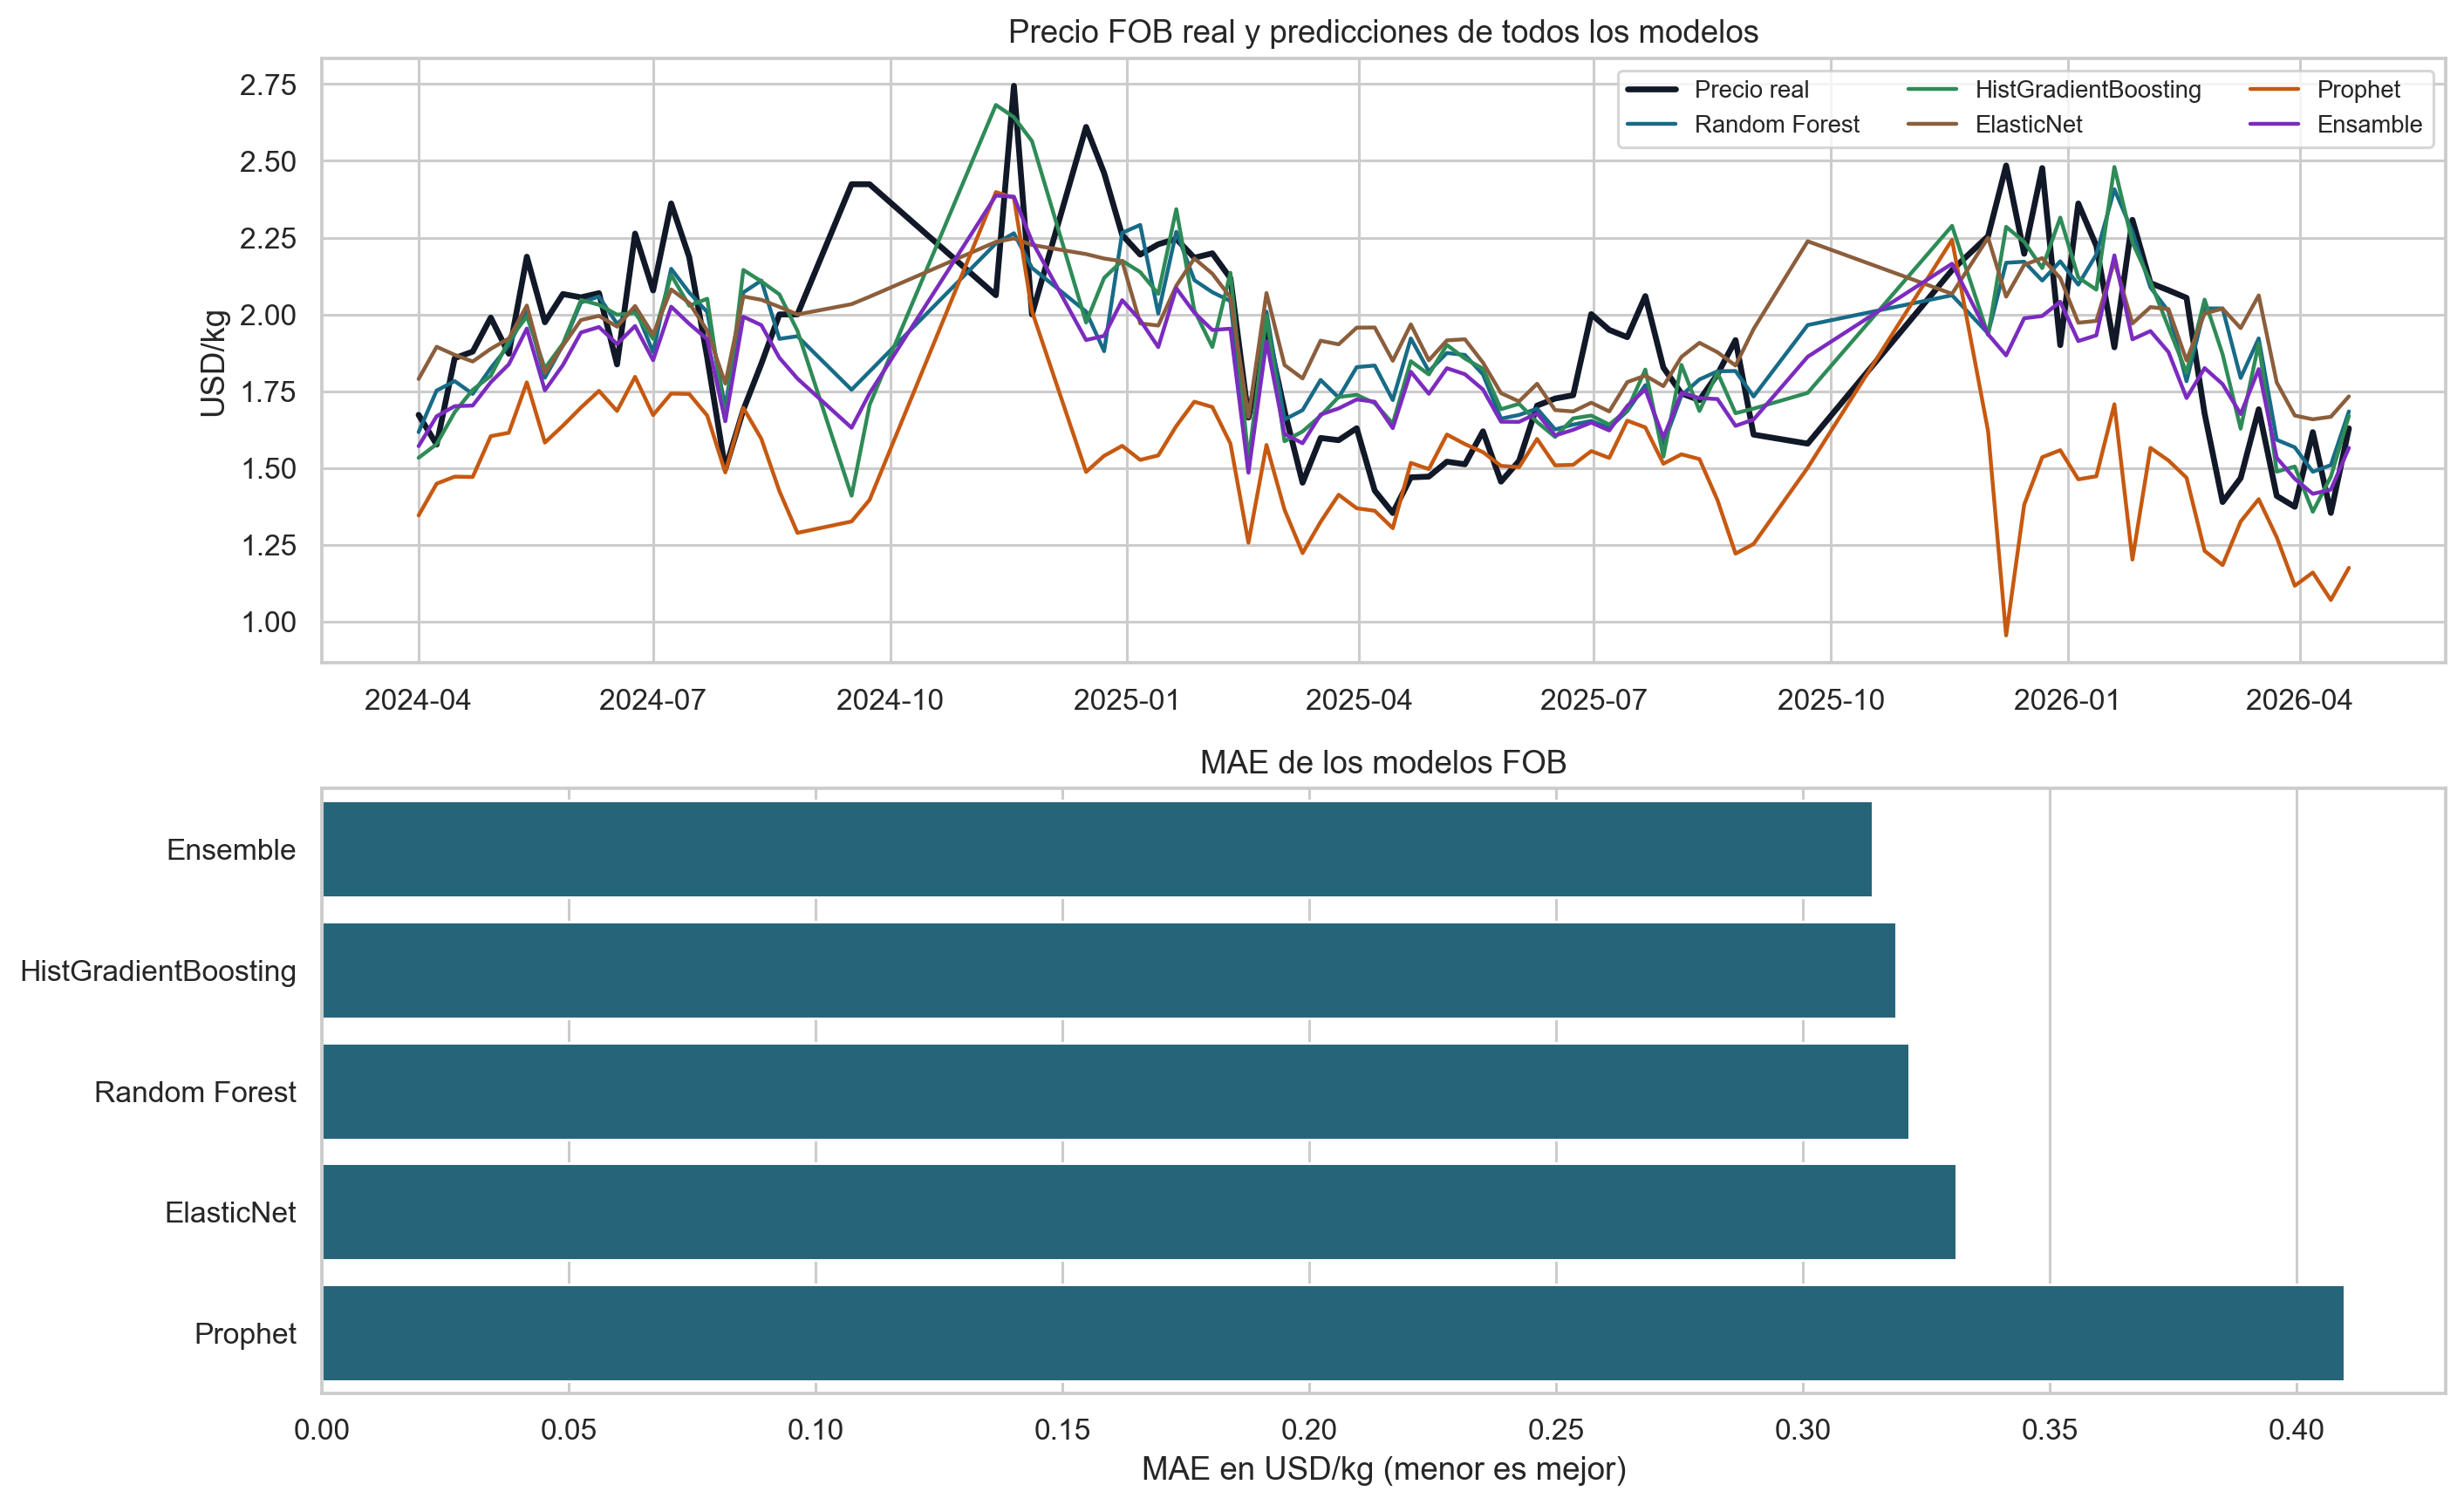
\includegraphics[width=\textwidth]{entrenamiento/outputs/figures/comparacion_completa_modelos_fob.png}
\end{figure}

En la parte superior de la Figura~\ref{fig:comparacion_completa_fob}, Random Forest, HistGradientBoosting y ElasticNet siguen de forma semejante la dirección del precio observado durante la mayor parte del bloque de prueba. Las diferencias se amplían en los cambios abruptos de finales de 2024 y finales de 2025. Prophet produce una trayectoria más suave y tiende a situarse por debajo del precio real en varios periodos de incremento, lo que explica su mayor MAE. El ensamble permanece generalmente dentro del grupo de predicciones y evita depender de la desviación puntual de un solo algoritmo.

La parte inferior de la figura confirma visualmente la jerarquía del MAE: el ensamble presenta la barra más corta, seguido por HistGradientBoosting y Random Forest. Sin embargo, las diferencias entre estos tres resultados son pequeñas. Por ello, la ventaja del ensamble debe interpretarse como una mejora incremental de estabilidad y no como una eliminación de la incertidumbre del precio.

\begin{figure}[H]
\caption{Resultados del ensamble para precio FOB}
\label{fig:resultado_fob_ensemble}
\centering
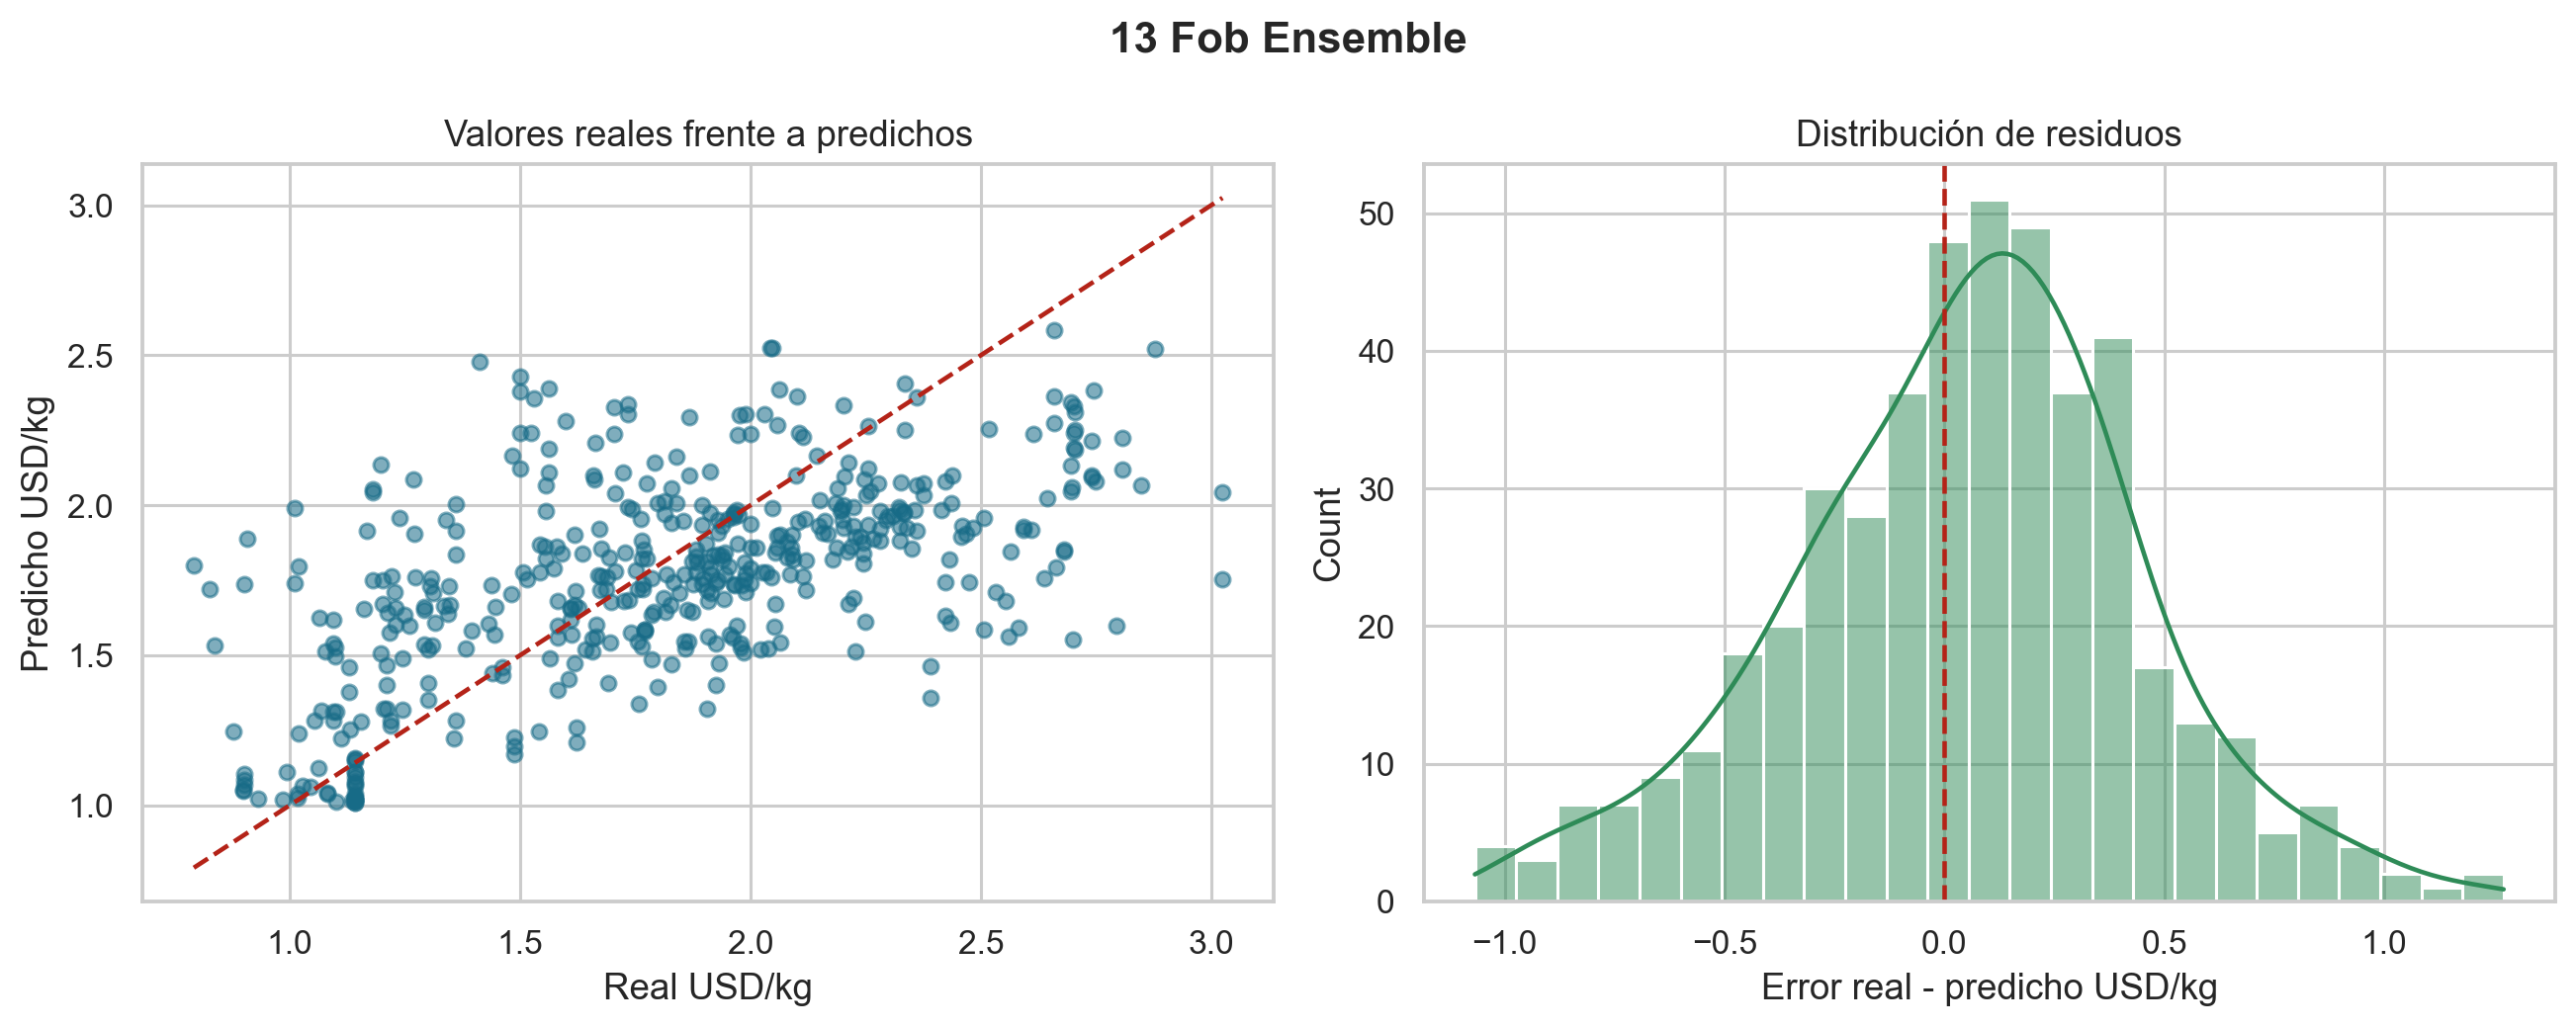
\includegraphics[width=\textwidth]{entrenamiento/outputs/figures/13_fob_ensemble_resultados.png}
\end{figure}

En el panel de valores reales frente a predichos de la Figura~\ref{fig:resultado_fob_ensemble}, la mayor concentración se ubica alrededor de la línea ideal, pero las predicciones presentan un rango más estrecho que los valores observados. Cuando el precio real es alto, varios puntos quedan debajo de la diagonal, lo que evidencia subestimación de picos; en algunos precios bajos ocurre el comportamiento contrario. Este patrón de regresión hacia el promedio explica que el sistema represente adecuadamente la tendencia general, pero no reproduzca completamente los extremos.

El histograma de residuos se concentra cerca de cero, aunque mantiene colas a ambos lados y una ligera acumulación de errores positivos. Puesto que el residuo se calculó como valor real menos valor predicho, los errores positivos representan subestimación. En términos prácticos, un MAE de 0,314 USD/kg continúa siendo relevante para la estimación de rentabilidad; por ello, la aplicación deberá presentar un rango de apoyo y advertir especialmente la posibilidad de subestimar semanas de precio elevado.

\section{Estimación del margen exportador}

\begin{table}[H]
\centering
\caption{Métricas de los modelos de margen}
\label{tab:resultados_margen}
\small
\begin{tabular}{lrrrr}
\toprule
\textbf{Modelo} & \textbf{MAE} & \textbf{RMSE} & \textbf{MAPE (\%)} & \textbf{$R^2$} \\
\midrule
Random Forest & \textbf{0,343} & \textbf{0,498} & 5,980 & \textbf{0,777} \\
HistGradientBoosting & 0,382 & 0,553 & 7,033 & 0,725 \\
ElasticNet & 0,392 & 0,553 & 7,094 & 0,724 \\
Prophet & 0,438 & 0,657 & 8,728 & 0,732 \\
\bottomrule
\end{tabular}
\end{table}

Random Forest presentó el mejor equilibrio entre MAE, RMSE, MAPE y capacidad explicativa, con un $R^2$ de 0,777. HistGradientBoosting obtuvo un MAE de 0,382 y representa una segunda alternativa no lineal. ElasticNet alcanzó un $R^2$ de 0,724 y funciona como referencia regularizada e interpretable. Prophet se evaluó con la misma partición de 438 registros de entrenamiento y 147 de prueba que los demás modelos; su $R^2$ de 0,732 confirma que captura una parte importante de la variación del margen, aunque sus errores absolutos son mayores.

El módulo de rentabilidad conservará las cuatro estimaciones. Random Forest proporcionará el valor central por su menor error, mientras que la diferencia entre los resultados de Random Forest, HistGradientBoosting, ElasticNet y Prophet se utilizará como indicador de sensibilidad. Una diferencia amplia entre modelos advertirá al usuario que la estimación económica es menos estable.

\begin{figure}[H]
\caption{Resultados de todos los modelos de margen exportador}
\label{fig:comparacion_completa_margen}
\centering
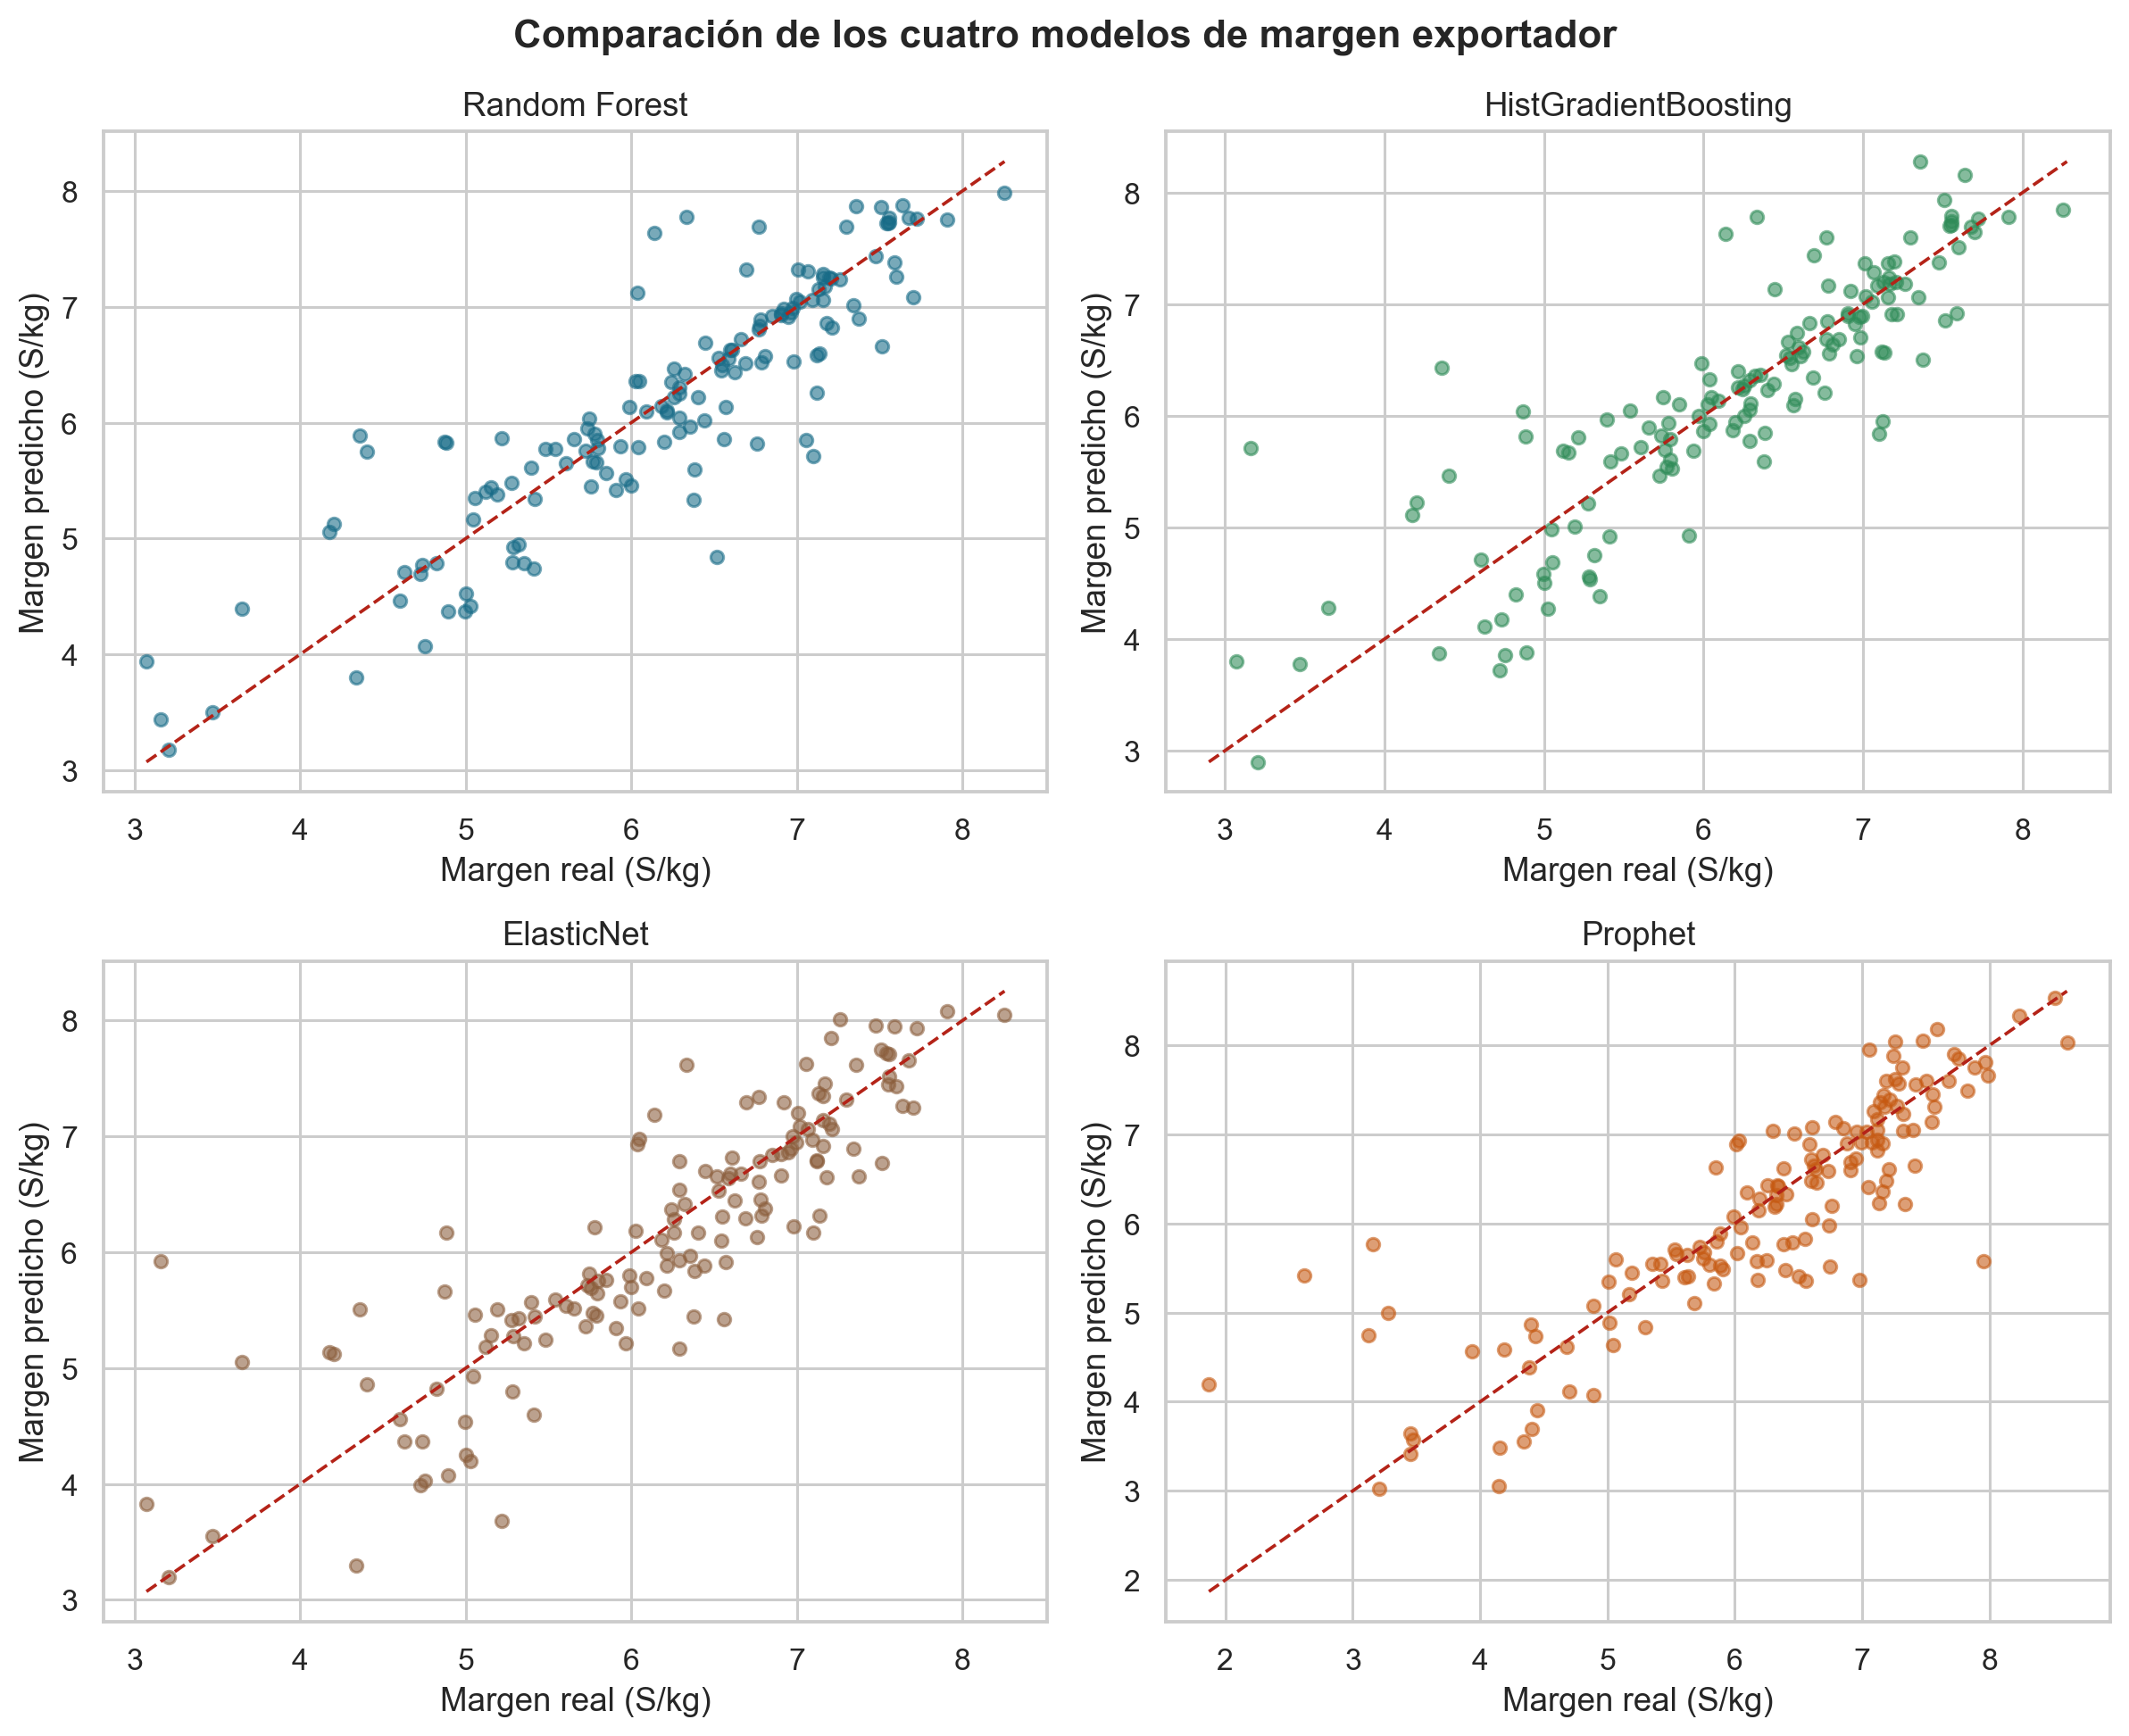
\includegraphics[width=\textwidth]{entrenamiento/outputs/figures/comparacion_completa_modelos_margen.png}
\end{figure}

La Figura~\ref{fig:comparacion_completa_margen} muestra que los cuatro modelos conservan una relación positiva clara entre margen real y margen estimado. Random Forest presenta la nube más próxima a la diagonal y una dispersión relativamente uniforme, en concordancia con su menor MAE y mayor $R^2$. HistGradientBoosting y ElasticNet ofrecen patrones muy parecidos: ambos representan bien la zona central, pero muestran mayor separación en márgenes bajos y en algunos valores superiores a S/ 7 por kilogramo.

Prophet también reproduce la dirección del margen y concentra numerosas observaciones cerca de la diagonal; sin embargo, aparecen desviaciones más pronunciadas en casos aislados de margen bajo y alto. Estos puntos influyen en su RMSE de 0,657. La coincidencia general entre los cuatro paneles respalda el uso conjunto como análisis de sensibilidad, mientras que la separación en los extremos justifica no comunicar una única cifra como si fuera exacta.

\section{Clasificación del riesgo de margen bajo}

\begin{table}[H]
\centering
\caption{Métricas de los modelos de riesgo}
\label{tab:resultados_riesgo}
\small
\begin{tabular}{lrrrr}
\toprule
\textbf{Modelo} & \textbf{Exactitud} & \textbf{Precisión} & \textbf{Recall} & \textbf{ROC AUC} \\
\midrule
Random Forest & 0,878 & 0,757 & 0,757 & 0,961 \\
HistGradientBoosting & 0,878 & \textbf{0,852} & 0,622 & 0,956 \\
Regresión logística & 0,878 & 0,711 & \textbf{0,865} & \textbf{0,965} \\
Prophet & 0,857 & 0,833 & 0,541 & 0,926 \\
\bottomrule
\end{tabular}
\end{table}

La regresión logística obtuvo el mayor recall y ROC AUC. Para un sistema de alerta resulta preferible detectar la mayor proporción posible de campañas con margen bajo, aun cuando aumenten algunos falsos positivos; por esa razón genera la alerta principal. Random Forest presenta un equilibrio entre precisión y recall; HistGradientBoosting aporta una alerta más conservadora por su mayor precisión; y Prophet permite observar el componente temporal del riesgo. No se reemplaza la regresión logística por Prophet, debido a que Prophet no es un clasificador nativo.

El simulador no elimina las salidas de los modelos con menor puntuación global. Las cuatro probabilidades se mostrarán internamente y podrán resumirse como nivel de acuerdo: acuerdo alto cuando todos clasifican el mismo escenario y acuerdo bajo cuando sus resultados divergen. De esta manera se aprovechan todos los modelos sin convertir una discrepancia algorítmica en una recomendación aparentemente segura.

\begin{figure}[H]
\caption{Comparación completa de todos los modelos de riesgo}
\label{fig:comparacion_completa_riesgo}
\centering
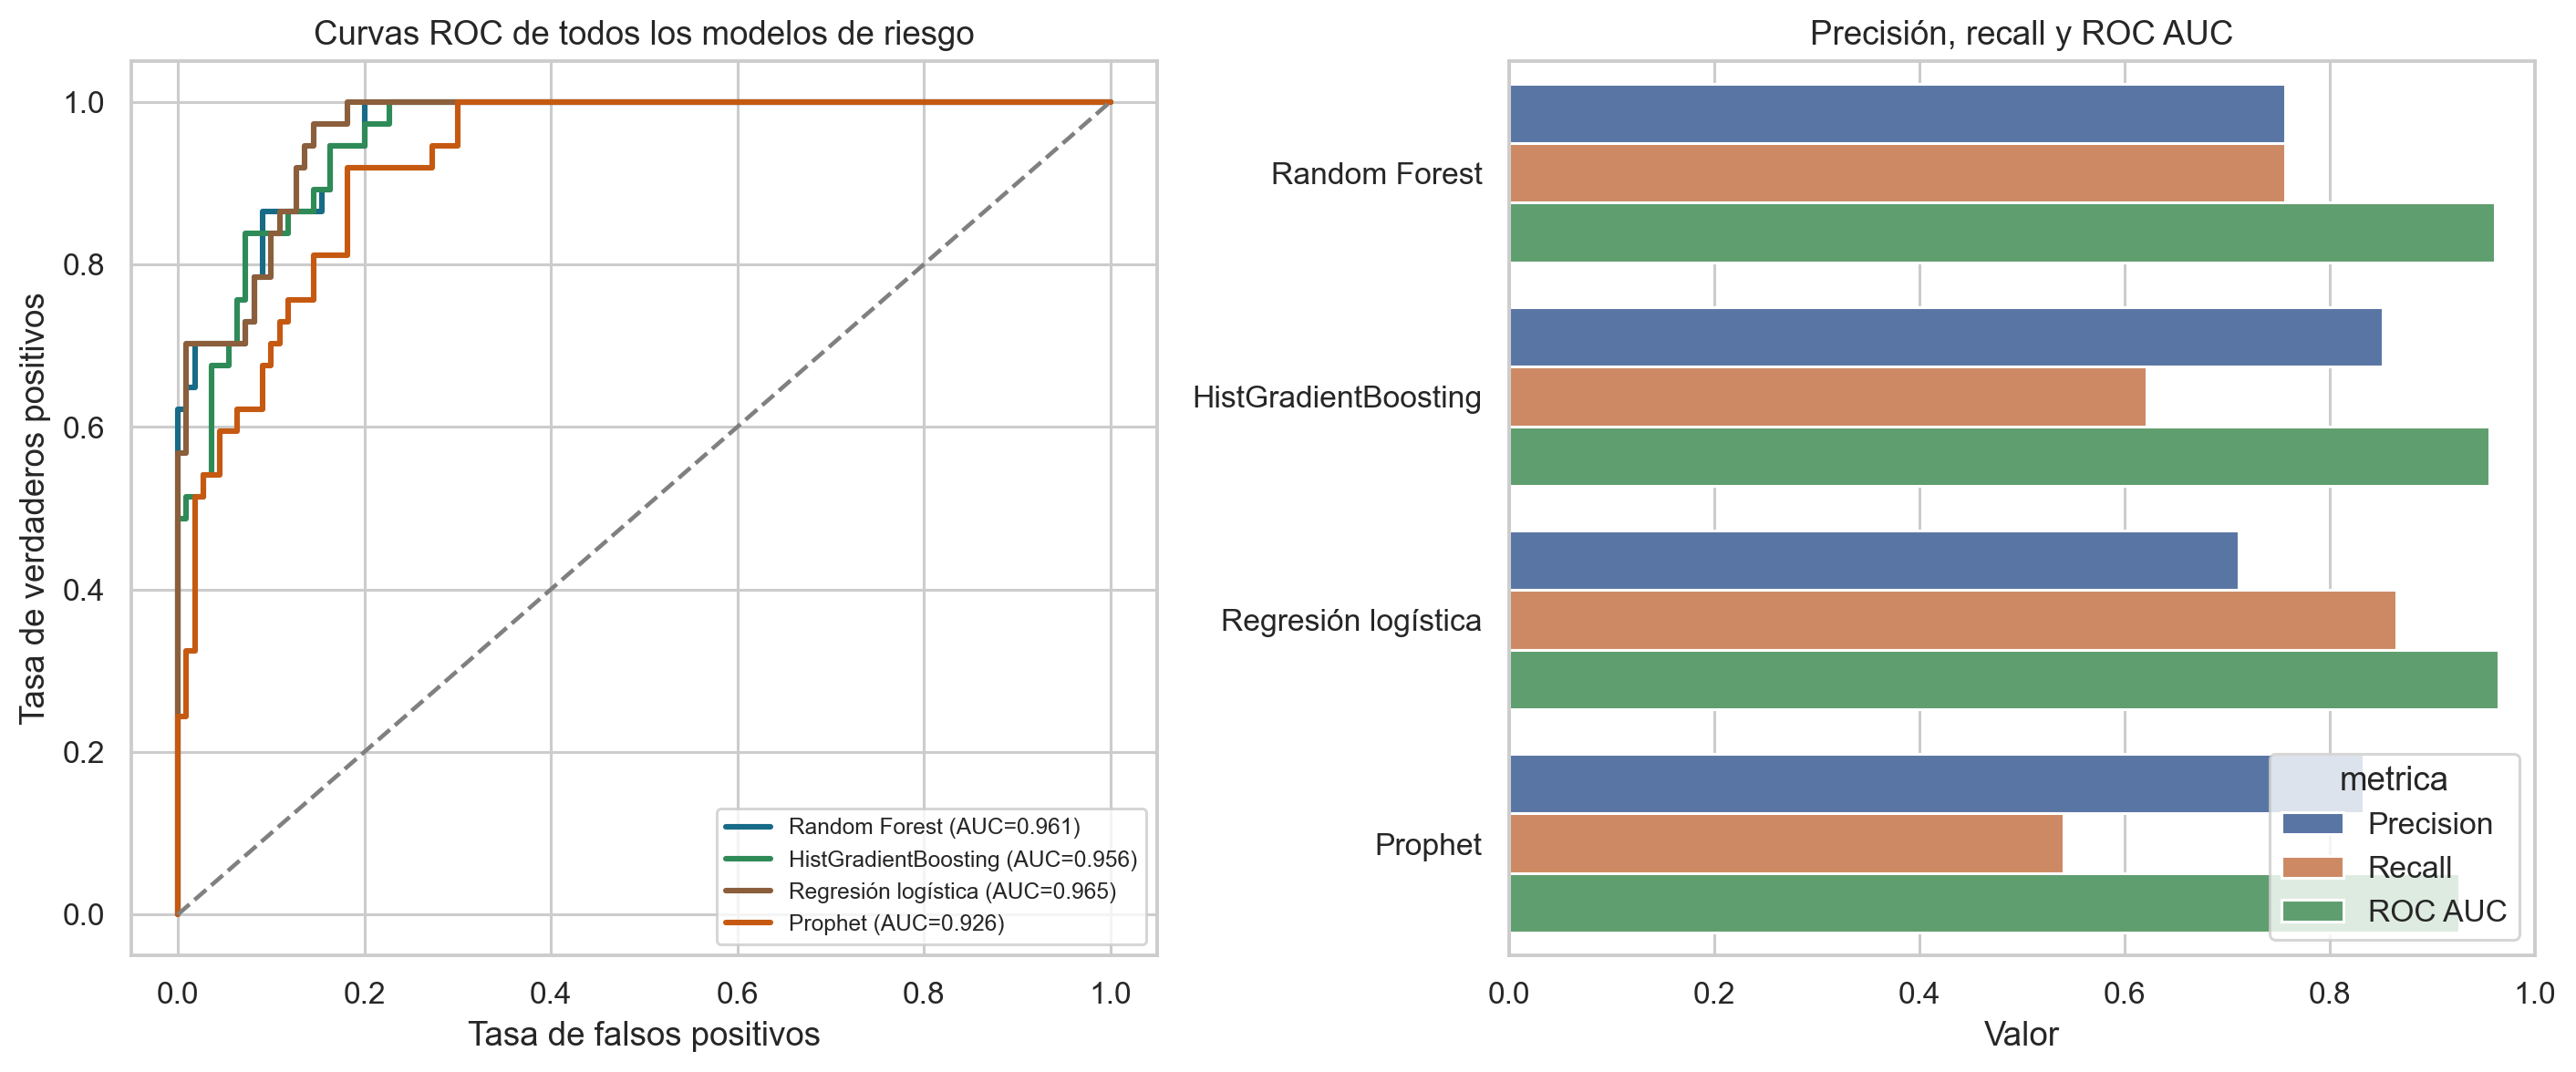
\includegraphics[width=\textwidth]{entrenamiento/outputs/figures/comparacion_completa_modelos_riesgo.png}
\end{figure}

Las curvas ROC de la Figura~\ref{fig:comparacion_completa_riesgo} se mantienen claramente por encima de la diagonal aleatoria, lo cual indica que los cuatro modelos poseen capacidad para ordenar observaciones normales y de riesgo. Las curvas de regresión logística, Random Forest e HistGradientBoosting son próximas entre sí y alcanzan rápidamente tasas altas de verdaderos positivos. Prophet conserva capacidad discriminante, pero su curva se separa de las tres primeras y su AUC de 0,926 confirma un desempeño comparativamente menor.

El panel de métricas evidencia que no existe un único ganador para todos los criterios. HistGradientBoosting alcanza la mayor precisión, por lo que emite menos alertas falsas, pero su menor recall implica que omite más casos reales de riesgo. La regresión logística presenta el mayor recall y ROC AUC, sacrificando parte de la precisión. Random Forest mantiene un equilibrio intermedio, mientras que Prophet combina precisión alta con el recall más bajo. Para la solución S-2, esta evidencia favorece utilizar la regresión logística como alerta preventiva y la coincidencia entre modelos como indicador adicional de confianza.

\section{Síntesis y limitaciones de los resultados}

Los resultados preliminares permiten proponer una arquitectura multimodelo completa. El precio FOB integra Random Forest, HistGradientBoosting, ElasticNet y Prophet mediante un ensamble. El margen conserva las cuatro estimaciones y utiliza Random Forest como valor central. El riesgo conserva Random Forest, HistGradientBoosting, regresión logística y Prophet, utilizando la regresión logística como alerta principal. El histórico interactivo compara observaciones y predicciones de todos los modelos, mientras que los reportes presentan métricas, dispersión y nivel de acuerdo. Por tanto, ningún algoritmo se excluye: cada uno cumple una función analítica o de contraste dentro de las soluciones.

Esta selección no implica que los modelos estén listos para uso productivo. El desempeño FOB continúa siendo moderado y requiere validación temporal por ventanas. El margen objetivo fue construido mediante el precio FOB, un tipo de cambio fijo de S/ 3,75 y costos agrícolas observados, por lo que existe una relación matemática fuerte que favorece a los modelos de margen. La separación de margen fue aleatoria y deberá complementarse con validación por año. La clase de riesgo representa el 25\,\% inferior de la distribución del margen y no equivale necesariamente a pérdida monetaria. Finalmente, las métricas evalúan capacidad técnica sobre datos históricos; todavía no demuestran una mejora real en decisiones de productores, aspecto que deberá evaluarse mediante el instrumento y la prueba piloto descritos en el Capítulo II.
